\section{Additional Evidence from the ACS and AHS}
\label{app:housing-stock}

In this appendix I report evidence from the ACS and the AHS that complements
the PSID event study of Section~\ref{sec:empirical-evidence}. Large homes are
mostly owned, and most large owned homes are held by older households. A
matched pseudo-panel and a twin design in the ACS give further
estimates of how housing changes with children.

\subsection{Large homes are owned}

Figure~\ref{fig:tenure-by-size} divides the 2023 housing stock in the
American Housing Survey (AHS) by number of bedrooms and tenure. Of the homes
with four or more bedrooms, 87\% are owner-occupied and 9\% are rented. Of
the homes with at most one bedroom, 13\% are owner-occupied and 74\% are
rented. In rooms, the unit I use in the rest of the paper, 43\% of
owner-occupied homes have seven or more rooms, against 7.5\% of rented homes.
The same gap appears among families. Owners with children live in 6.8 rooms
on average, and renters with children in 5.2. Of renter households with
children, 48.7\% live in homes with at most two bedrooms, against 7.4\% of
owner households with children. These shares describe the homes that
households occupy, and they say nothing directly about the homes on offer.
Still, in the existing stock a family that wants a large home usually has to
buy one.

\begin{figure}[ht]
\centering
\includegraphics[width=0.7\linewidth]{figures/tenure_by_bedrooms_ahs2023_v2.pdf}
\caption{Tenure of the housing stock by number of bedrooms, AHS 2023}
\label{fig:tenure-by-size}
\par\smallskip
\begin{minipage}{0.92\linewidth}
\footnotesize\textit{Notes:} Each bar divides the housing units with the
stated number of bedrooms into owner-occupied units, units rented for cash
and vacant units, in \%. Units occupied without payment of cash rent and
units whose occupants have a usual residence elsewhere are excluded. Weighted
by the housing-unit weight. Source: American Housing Survey 2023, national
public-use file.
\end{minipage}
\end{figure}

\subsection{Older households hold the large homes}

Figure~\ref{fig:large-homes} divides the owner-occupied homes with six or
more rooms in the 2023 American Community Survey (ACS) by the age of the
householder and by whether a child of the householder younger than 18 lives
in the home. Households aged 60 to 85 without children at home hold 42.5\% of
these homes, and households aged 40 to 59 without children another 21.6\%.
Households aged 22 to 39 with children hold 11.2\%. Across all ages, 70.2\%
of the large owned homes house no child of the householder, against 73.4\% of
all households. Large owned homes thus house children only slightly more
often than homes in general, and their owners differ mainly in age. This
concentration is what \citet{coven2026} calls the intergenerational
allocation of housing. For a young
family, it means that the existing large homes come on the market mainly when
older households sell or leave them.

\begin{figure}[ht]
\centering
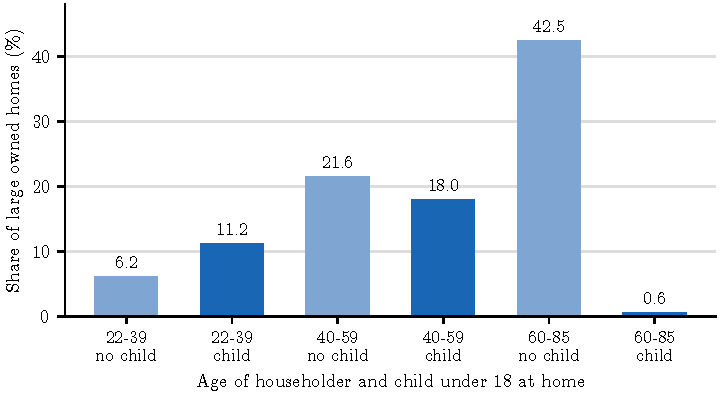
\includegraphics[width=0.7\linewidth]{figures/large_homes_by_age_children_acs2023_national.pdf}
\caption{Who holds the large owner-occupied homes, ACS 2023}
\label{fig:large-homes}
\par\smallskip
\begin{minipage}{0.92\linewidth}
\footnotesize\textit{Notes:} Share of owner-occupied homes with six or more
rooms held by each group, in \%. The six shares sum to 100\%. Groups are
defined by the age of the householder and by whether an own child of the
householder younger than 18 lives in the household. Householders aged 22 to
85, weighted by the household weight; 664,243 households. Source: American Community Survey 2023.
\end{minipage}
\end{figure}

\subsection{ACS matched pseudo-panel}
\label{app:acs-pseudo-panel}

The PSID estimates of Section~\ref{sec:empirical-evidence} follow the same
people over time, but they rest on a limited sample size, although
representative. To corroborate them, I estimate the housing response to the first
birth in the ACS, which surveys about three
million people each year. The ACS is a repeated cross-section with no birth
histories, so it does not show a mother's home before her first child. I
therefore use the pseudo-event study design of
\citet{klevenGeographyChildPenalties2025}. Kleven develops it to estimate
child penalties in earnings and employment, and shows that it reproduces the
estimates of event studies on panel data. The design has three steps. First,
I date each mother's first birth from the age of her oldest own child in the
household. Second, I build the years before the birth by matching each new
mother to childless women observed one to five years earlier, who were then
her age and share her education, marital status, race and state. Third, I
estimate an event study on the resulting synthetic panel. I follow his sample
definitions, matching cells and matching rule, and add one headship
restriction that housing outcomes require, described below.

\subsubsection*{Sample.}
I use the ACS one-year files for 2005--2019, for all states and the District
of Columbia, and keep women. The ACS lists the own children of each person
who live in the same household, with the age of the oldest. For a woman with
own children in the household, I date her first birth to the survey year
minus the age of her oldest own child, so her event time $\tau$ equals that
age. Mothers enter the sample at $\tau = 0, \dots, 10$ if their age at the
first birth is between 25 and 45. Childless women are women with no own
child in the household.

Rooms and tenure in the ACS describe the dwelling, not the person. For a
woman who lives in her parents' home, they describe the parents' home. As in
the PSID (Appendix~\ref{app:empirical-data}), I keep women who are the
householder, the householder's spouse, or the householder's unmarried
partner, and who live in a household rather than in group
quarters.\footnote{The ACS householder is the person in whose name the home
is owned or rented, and plays the role of the PSID reference person. In the
IPUMS files, these are the codes 1 and 2 of \texttt{RELATE}, the code 1114
of \texttt{RELATED}, and the codes 1, 2 and 5 of \texttt{GQ}.} The
restriction applies to mothers and to childless women alike.

\subsubsection*{Matching.}
Let mother $i$ be observed at $\tau=0$ in survey year $t$, at age $a$, with
characteristics $X_i$. These are education (less than high school, high
school, some college, college degree), marital status (married with spouse
present, married with spouse absent or separated, divorced, widowed, never
married), race and ethnicity (white non-Hispanic, Black non-Hispanic, other
non-Hispanic, Hispanic) and state of residence. For each $n = 1,\dots,5$, the
matches of $i$ at event time $-n$ are all childless women observed $n$ years
earlier, $n$ years younger, and in the same cell,
\begin{equation}
\mathcal{M}_{i,n} = \bigl\{\, j \,:\, \text{$j$ childless},\;
t_j = t - n,\; a_j = a - n,\; X_j = X_i \,\bigr\}.
\end{equation}
Each $j \in \mathcal{M}_{i,n}$ enters the panel as a synthetic observation of
mother $i$ at $\tau = -n$, with weight
\begin{equation}
\omega_{ij} = \frac{w_j}{k_{i,n}}, \qquad k_{i,n} = \left| \mathcal{M}_{i,n} \right|,
\end{equation}
where $w_j$ is the ACS person weight of $j$. The matching is exact. It
minimizes no distance and uses no propensity score. Every childless woman in
the mother's cell is a match, all ties are kept, and matching is with
replacement, as in \citet{klevenGeographyChildPenalties2025}, who implements
it with the \texttt{Matching} package of \citet{sekhonMatching2011}. The
factor $1/k_{i,n}$ makes the $k_{i,n}$ matches of mother $i$ at lag $n$ count
together as a single observation, with the average survey weight of the
childless women in her cell. A childless woman can serve as a match for
several mothers and at several lags, and each match is a separate record.

For example, take a mother observed in the 2015 ACS at age 30, with a
newborn first child, a college degree, married with her spouse present, white
non-Hispanic and living in New York. Her matches at $\tau=-1$ are all
childless women in the 2014 ACS who are 29 and have the same education,
marital status, race and ethnicity and state. Two years before the birth, her matches are the women aged 28 in the 2013
ACS with the same characteristics, and the same rule gives her matches back
to five years before the birth. I keep her characteristics as observed in
2015 at every lag. If there is no matching cell, there is no record at that lag, so the
baseline panel is unbalanced. I observe housing only in the ACS 2005--2019
files, so matches from earlier years drop out as well, and mothers observed
early in the sample appear at fewer lags. Column (4) of
Table~\ref{tab:app-acs-pseudo} keeps only mothers with matches at every lag.\footnote{I apply the headship restriction to the
matched panel and recount $k_{i,n}$ over the women who meet it. With exact
matching, the records and weights are the same as if the restriction were
applied before matching.}

The design assumes that, within a cell, childless women at age $a-n$ in year
$t-n$ live on average as the future mothers lived at that age and year
\citep[Assumption 3]{klevenGeographyChildPenalties2025}.

\subsubsection*{Estimation.}
I consider three housing outcomes, all from the household record: rooms
(capped at nine, with codes that are not a count set to missing), bedrooms
(capped at five), and an indicator for living in an owner-occupied dwelling
(one if the home is owned or being bought, zero if rented). For a record $r$
with event time $\tau_r$, I estimate
\begin{equation}
Y_r = \sum_{k \neq -2} \beta_k \, \mathbf{1}\{\tau_r = k\} + \alpha_{a_r} +
\gamma_{s_r} + \delta_{y_r} + \varepsilon_r ,
\end{equation}
where $k$ runs from $-5$ to $10$, and $\alpha_{a_r}$, $\gamma_{s_r}$ and
$\delta_{y_r}$ are fixed effects for age, state and survey year. Mothers'
records are weighted by the ACS person weight and matched records by
$\omega_{ij}$. Standard errors are clustered by ACS household, since a childless woman
matched to several mothers or lags appears in several records. The estimate I
report is $\beta_3 - \beta_{-1}$, the change in housing between one year
before and three years after the first birth. Table~\ref{tab:app-acs-sample} describes the panel.

\begin{table}[ht]
\centering
\caption{ACS pseudo-panel, sample}
\label{tab:app-acs-sample}
\small
\begin{tabular}{@{}lrr@{}}
\toprule
 & Householder, spouse & All \\
 & or partner & women \\
\midrule
Mothers at $\tau = 0$ & 107{,}565 & 116{,}857 \\
\quad with matches at $\tau = -1$ & 92{,}559 & 102{,}097 \\
\quad with matches at $\tau = -3$ & 78{,}275 & 86{,}834 \\
\quad with matches at $\tau = -5$ & 61{,}953 & 69{,}216 \\
Records in the regression & 11{,}254{,}007 & 14{,}155{,}689 \\
Households (clusters) & 2{,}139{,}934 & 2{,}765{,}428 \\
\bottomrule
\end{tabular}
\par\smallskip
\begin{minipage}{0.75\linewidth}
\footnotesize\textit{Notes:} Women with a first birth at ages 25 to 45, ACS
2005--2019. Matches at $\tau=-n$ count mothers with at least one matched
childless woman with housing data at that lag. Records are mothers at
$\tau = 0,\dots,10$ and matched childless women at $\tau = -5,\dots,-1$, for
rooms.
\end{minipage}
\end{table}

\subsubsection*{Results.}
Figure~\ref{fig:app-acs-pseudo} plots the coefficients $\beta_k$ and
Table~\ref{tab:app-acs-pseudo} reports $\beta_3 - \beta_{-1}$. Between one
year before and three years after the first birth, rooms rise by 0.59, from
5.21 at $\tau=-1$, bedrooms by 0.41, and the share in an owner-occupied
dwelling by 4.6 percentage points, from 54.6 percent. The coefficients before
the birth are flat. Rooms at $\tau=-5$ are 0.01 above $\tau=-2$.

Column (2) keeps all women, whatever their headship status, as in
\citet{klevenGeographyChildPenalties2025}. Rooms then rise by 0.49 and
ownership by 3.3 percentage points, and rooms rise before the birth, by 0.06
between $\tau=-5$ and $\tau=-2$. In this sample, 8.5 percent of the matched
childless women at $\tau=-1$ live in a home where they are a child of the
householder, against 5.7 percent of mothers at $\tau=+3$. Those homes have
6.35 rooms on average, against 5.17 for the homes of householders.

Columns (3) and (4) restrict the main sample. Column (3) keeps first births
at ages 30 to 45, and rooms rise by 0.79. Column (4) keeps mothers with
matches at every lag from $-5$ to $-1$, and rooms rise by 0.55. The fixed
effects matter mostly for ownership. Without fixed effects, ownership rises by
13.6 percentage points, and with age fixed effects only by 5.8, since
ownership rises steeply with age at these ages. Rooms rise by 0.89 without
fixed effects and by 0.65 with age fixed effects only.

\begin{table}[ht]
\centering
\caption{Housing around the first birth, ACS pseudo-panel}
\label{tab:app-acs-pseudo}
\small
\begin{tabular}{@{}lrrrr@{}}
\toprule
 & (1) & (2) & (3) & (4) \\
 & Householder, & All & First birth & Matches \\
 & spouse or partner & women & at 30--45 & at every lag \\
\midrule
Rooms & 0.59 & 0.49 & 0.79 & 0.55 \\
 & (0.008) & (0.008) & (0.012) & (0.009) \\
Bedrooms & 0.41 & 0.34 & 0.50 & 0.40 \\
 & (0.005) & (0.004) & (0.006) & (0.005) \\
Owner-occupied (pp) & 4.6 & 3.3 & 9.0 & 3.2 \\
 & (0.2) & (0.2) & (0.3) & (0.2) \\
\addlinespace
Rooms at $\tau=-1$ & 5.21 & 5.41 & 5.38 & 5.25 \\
Owner-occupied at $\tau=-1$ (\%) & 54.6 & 57.8 & 60.5 & 54.2 \\
Mothers at $\tau=0$ & 107{,}565 & 116{,}857 & 62{,}480 & 57{,}061 \\
Records & 11{,}254{,}007 & 14{,}155{,}689 & 7{,}497{,}375 & 9{,}331{,}335 \\
\bottomrule
\end{tabular}
\par\smallskip
\begin{minipage}{0.92\linewidth}
\footnotesize\textit{Notes:} Coefficient at $\tau=+3$ minus coefficient at
$\tau=-1$, with age, state and survey-year fixed effects. Standard errors
clustered by ACS household in parentheses. Values at $\tau=-1$ are
weighted means before the regression. Columns (1), (3) and (4) keep
householders, spouses and unmarried partners; column (2) keeps all women.
ACS 2005--2019.
\end{minipage}
\end{table}

\begin{figure}[ht]
\centering
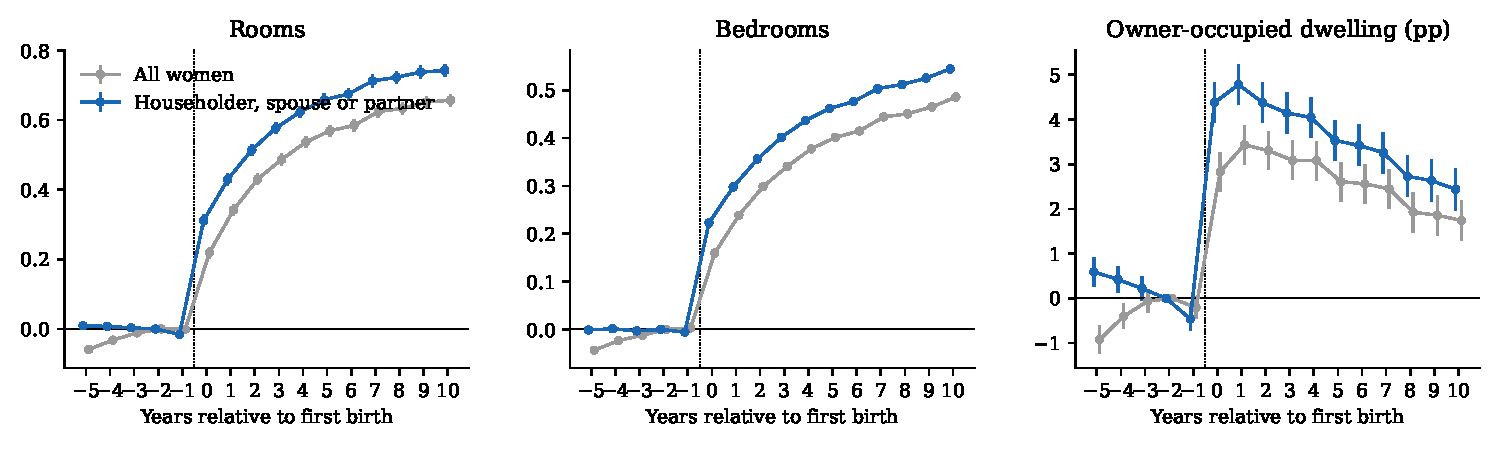
\includegraphics[width=\linewidth]{figures/acs_pseudo_panel_event_study.pdf}
\caption{Housing around the first birth, ACS pseudo-panel}
\label{fig:app-acs-pseudo}
\par\smallskip
\begin{minipage}{0.92\linewidth}
\footnotesize\textit{Notes:} Coefficients $\beta_k$ relative to $\tau=-2$,
with 95 percent confidence intervals clustered by ACS household. The blue line
keeps householders, spouses and unmarried partners, and the grey line keeps
all women.
\end{minipage}
\end{figure}

\subsubsection*{Comparison with the PSID.}
In the PSID sample of women, rooms are 1.03 (0.07) higher three to four
years after the first birth than two to three years before it
(Table~\ref{tab:app-rooms-path}, column 2), against 0.59 in the ACS between
$\tau=-1$ and $\tau=+3$. Hence, the results are qualitatively similar,
although quite different quantitatively. There are some important
differences worth outlining. First, the PSID compares the same women over
time, while in the ACS the years before the birth are other women, matched on
a set of observables. Second, in the PSID I date the first birth from birth
histories, while in the ACS I do it from the oldest own child in the
household, since the ACS asks only whether a woman gave birth in the past
twelve months. The oldest own child misses children living elsewhere and does
not separate biological from other children. Finally, the PSID windows are
two years wide, while the ACS compares single years.

\subsection{Twin births}
\label{app:twins}

The pseudo-panel compares mothers with other women. Twin births give a
comparison among mothers. A woman whose first birth is a twin birth has a
second child at once, while other mothers choose whether and when to have
one. Comparing their housing gives the effect of a second child, under the
assumption that a twin birth affects housing only through the number of
children.

\subsubsection*{Sample and design.}
I use women aged 21 to 35 in the ACS one-year files for 2005--2019 whose
oldest own child in the household is aged 0 to 5. The household roster records the children who
live with the mother, not all the children she has borne, and does not
separate biological from step or adoptive children.

The instrument is an indicator that the two oldest own children are recorded
at the same age. Since the ACS records age in whole years, without the
quarter of birth, the indicator also counts siblings born less than a year
apart, and it is a proxy for a twin birth. The treatment is an indicator for
a second own child in the household. I estimate the effect by two-stage least
squares, with fixed effects for the mother's age at the first birth, her race
and ethnicity, the survey year and the age of the oldest child. The
regressions are weighted by the ACS person weight, and standard errors are
clustered by ACS household.

I report two samples. The first keeps all mothers. The second keeps, as in
Appendix~\ref{app:acs-pseudo-panel}, mothers who are the householder, the
householder's spouse or the householder's unmarried partner. A twin birth
lowers the probability that the mother is in this group by 2.9 percentage
points (0.4), so the second sample conditions on an outcome of the
instrument. I therefore use all mothers as the main sample and the second as
a check.

\subsubsection*{Results.}
Table~\ref{tab:app-twins} reports the estimates and
Figure~\ref{fig:app-twins} plots them by the age of the oldest child. Among
all mothers, a twin first birth raises the probability of a second child in
the household by 66 percentage points, with a first-stage $F$ statistic
above 77,000. The first stage is below one since many mothers of one child
have a second within a few years, and it falls to 35 points when the oldest
child is five. A second child raises rooms by 0.50, bedrooms by 0.33 and the
share in an owner-occupied dwelling by 4.7 percentage points. The effect
grows with the age of the children. When the oldest child is three, a second
child adds 0.63 rooms and 3.1 points of ownership. When the oldest child is
five, it adds 1.10 rooms and 15.1 points. Among householders, spouses and
partners, the estimates are close, with 0.45 rooms and 4.5 points.

\begin{table}[ht]
\centering
\caption{Effect of a second child on housing, twin births in the ACS}
\label{tab:app-twins}
\small
\setlength{\tabcolsep}{4pt}
\begin{tabular}{@{}lrrrrrr@{}}
\toprule
 & \multicolumn{3}{c}{All mothers} & \multicolumn{3}{c}{Householder, spouse or partner} \\
\cmidrule(lr){2-4}\cmidrule(l){5-7}
 & (1) & (2) & (3) & (4) & (5) & (6) \\
Age of oldest child & 0--5 & 3 & 5 & 0--5 & 3 & 5 \\
\midrule
First stage (pp) & 66.2 & 52.5 & 34.8 & 64.1 & 48.7 & 31.3 \\
 & (0.2) & (0.2) & (0.2) & (0.3) & (0.3) & (0.2) \\
Rooms & 0.50 & 0.63 & 1.10 & 0.45 & 0.62 & 1.09 \\
 & (0.03) & (0.08) & (0.12) & (0.03) & (0.09) & (0.14) \\
Bedrooms & 0.33 & 0.40 & 0.67 & 0.30 & 0.39 & 0.65 \\
 & (0.01) & (0.04) & (0.07) & (0.02) & (0.05) & (0.08) \\
Owner-occupied (pp) & 4.7 & 3.1 & 15.1 & 4.5 & 2.0 & 12.5 \\
 & (0.7) & (2.2) & (3.3) & (0.7) & (2.4) & (3.8) \\
\addlinespace
Mothers & 857{,}607 & 147{,}986 & 142{,}101 & 735{,}796 & 126{,}812 & 122{,}867 \\
\bottomrule
\end{tabular}
\par\smallskip
\begin{minipage}{0.95\linewidth}
\footnotesize\textit{Notes:} Two-stage least squares. The instrument is an
indicator that the two oldest own children are recorded at the same age, and
the treatment is an indicator for a second own child in the household. The
first stage is in percentage points. Fixed effects for the mother's age at
the first birth, race and ethnicity, survey year and age of the oldest child.
Standard errors clustered by ACS household in parentheses. Women aged 21 to
35, ACS 2005--2019.
\end{minipage}
\end{table}

\begin{figure}[ht]
\centering
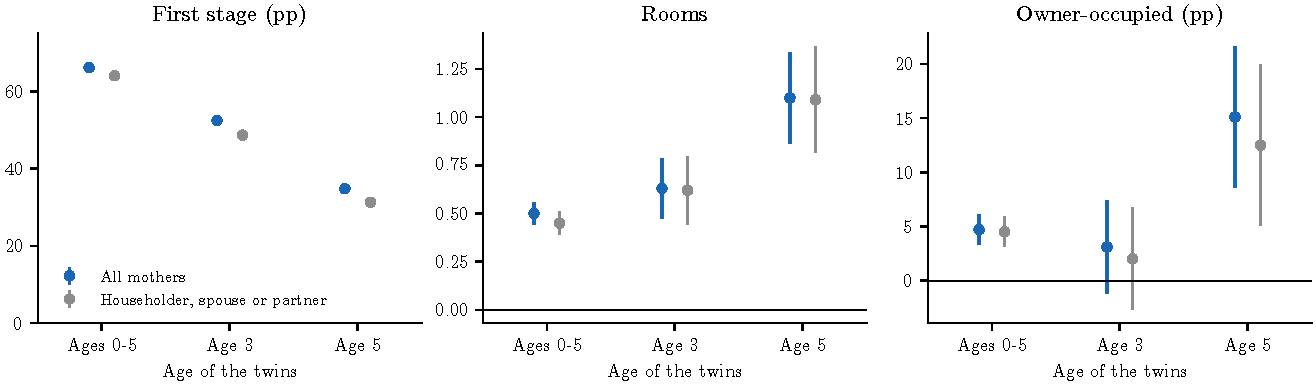
\includegraphics[width=\linewidth]{figures/twins_iv_by_child_age.pdf}
\caption{Effect of a second child on housing, twin births in the ACS}
\label{fig:app-twins}
\par\smallskip
\begin{minipage}{0.92\linewidth}
\footnotesize\textit{Notes:} First stage and two-stage least squares
estimates from Table~\ref{tab:app-twins}, by the age of the oldest child,
with 95 percent confidence intervals clustered by ACS household. Blue dots
keep all mothers, and grey dots keep householders, spouses and unmarried
partners.
\end{minipage}
\end{figure}

\subsection{Data on the housing stock}

The stock facts use the national public-use household file of the 2023
American Housing Survey, weighted by the housing-unit weight. Tenure has
three occupied categories: owned, rented for cash, and occupied without
payment of cash rent. Shares within a tenure use all units of that tenure as
the denominator. The share of homes with seven or more rooms that are rented
uses all occupied units of that size instead. It is 8.2\% when the
denominator contains owned and cash-rented units, and 8.1\% when it also
contains units occupied without cash rent and units with unreported tenure.
Bedrooms and rooms are different measures. I report bedrooms for comparison
with other work, and rooms because rooms are the outcome in the PSID and the
ACS and the unit of the model. Mean rooms among households with children are
computed over households with at least one child present.
